\section{Bericht}

\subsection{Einleitung}
Ziel dieses Versuchs ist es die in $Versuch\ 2$ errechneten Werte für den PID-Regler in den vorhandenen Quellcode einzufügen und so ein funktionierendes System zu erlangen. Zusätzlich müssen die Werte für $MIDPOS$ und $DELTA$ berechnet und der Willkommenstext auf der LCD-Anzeige gändert werden. 

\subsubsection{Verwendung von OCR3A}
$OCR3A$ ist das Timer Output Compare Register. Wenn der Zähler des timer clock cycle (Register $TCNT3$) den Wert des Registers $OCR3A$ erreicht, wird ein Interrupt erzeugt. \\
Im Register $OCR3A$ ist die Pulslänge für die errechnete nächste anzusteuernde Position hinterlegt.\\
\begin{equation}
OCR3A = (unsigned\ int) (MIDPOS - (int)(beta \cdot DELTA))
\end{equation}
Zu Beginn des Versuchs wird die Pulsweite auf die Mittelposition ($MIDPOS=375$ entspricht einer Pulsweite von $1,5ms$) gesetzt, um die Fläche zu kalibrieren. (Näheres siehe "1.1.2 Berechnung von MIDPOS").

\subsubsection{Berechnung von MIDPOS}
Der richtige $MIDPOS$ Wert gibt an, wann die Fläche vollkommen horizontal steht. Zur Berechnung von MIDPOS benutzten wir folgende Formel: \\
\begin{equation}
MIDPOS  = Frequenz / Prescaler \cdot Pulslaenge
\end{equation}
Die Frequenz ist mit $16 MHz$ gegeben. Der Prescaler-Wert ist im Register $TCCR3B$ auf den Wert $0b00000011$ gesetzt. Mit Hilfe des Datenblatts\footnote{http://www.atmel.com/Images/doc2467.pdf} kann diese Bitfolge auf den Wert $64$ dekodiert werden. Die Pulslänge der PWM (Pulsweitenmodulation) für eine horizontaler Lage ist in der Aufgabenstellung erwähnt und liegt bei $1,5 ms$.\\
Das Ergebnis unserer Berechnung ergibt $MIDPOS = 375$. Allerdings ist die Fläche nach dem Setzen von $MIDPOS$ auf den errechneten Wert nicht vollständig horizontal. Der Wert muss auf $MIDPOS = 355$ angepasst werden, damit unser Modell in der Waage ist. \\ 
Zu beachten ist, dass der Wert von $MIDPOS$ eventuell vor jeder Versuchsdurchführung neu angepasst werden muss, um zum Beispiel ein Schiefstehen des Tisches oder ähnliches auszugleichen.

\subsubsection{Berechnung von DELTA}
$DELTA$ ist die Differenz zwischen der maximalen linken oder rechten Position der Fläche und der mittleren Position ($MIDPOS$). Für die Berechnung des Wertes von $DELTA$ verwenden wir die folgende Formel
\begin{equation}
DELTA = (Frequenz / Prescaler \cdot Pulslaenge) - MIDPOS
\end{equation}
Für den Wert der Pulslänge muss diesmal allerdings $2 ms$ verwendet werden, da wir den Wert für die maximale rechte Position der Fläche benötigten. Von diesem Wert ziehen wir $MIDPOS$ ab, um die Differenz zu erhalten. Da der errechnete Wert von $MIDPOS$ um $20$ verringer wurde, müssen nun auch die Werte von der rechten und linken Position angepasst werden (um $20$ verringert). Somit kommen wir auf das Ergebnis $DELTA = 125$.

\subsubsection{Willkommens-Anzeige}
Die Willkommensnachricht auf der LCD Anzeige ist in der Datei $HMI.c$ in Zeile 260 festgelegt und kann einfach mit der richtigen Gruppennummer angepasst werden.

\subsubsection{PID Implementation}
Die Implementierung des PID-Reglers erfolgt in der Datei $PID.c$. Wir verwenden folgende Summenformel für den PID-Regler:
\begin{multline}
y = (proportional \cdot error) + (integral \cdot errorSum \cdot sampleTime) + \\
(derivative \cdot (error - errorLast) / sampleTime)
\end{multline}
Die Werte für $proportional$, $integral$ und $derivative$ sind die Faktoren für den P-, I- und D-Teil des Reglers. $error$ beschreibt den aktuellen Fehler (Sollwert minus Istwert). $errorSum$ ist die Summe aller bisherigen Fehler. $errorLast$ beschreibt den vorherigen Fehler. \\
Die $sampleTime$ haben wir auf $18 ms$ ($0,018s$) gesetzt, da die Ansteuerung des Servo-Motors alle $18 ms$ erfolgt. \\
Im $Versuch\ 2$ haben wir den PID-Regler simuliert. Leider können die Werte aus der Simulation nicht übernommen werden. Ein Grund dafür ist, dass in der Simulation ein kontinuierlicher PID simuliert wird, wir am Modell jedoch einen diskreten PID vorfinden. Außerdem werden in der Simulation Einflüsse wie zum Beispiel die nicht perfekte Rundheit des Balls, die Trägheit des Servo-Motors und so weiter ignoriert. \\
Nach längerem Kalibrieren kommen wir auf folgende Werte: \\
$proportional = 0,19$, $integral =0,018$ und $derivative = 0,51$


\subsubsection{Vergleich der Ergebnisse mit Versuch 2}
Im Vergleich zu $Versuch\ 2$ benötigten wir beim eigentlichen Modell vollkommen andere PID-Werte. Ein Grund dafür ist, dass wir in Versuch 2 ein kontinuierliches System simuliert haben, in Versuch 3 aber mit einem diskreten System arbeiten. Der Unterschied ist, dass bei einem diskreten PID die $sampleTime$, also eine Verzögerungszeit, mit eingerechnet werden muss. Dadurch ändert sich die Formel des Reglers.\\
Außerdem werden, wie oben bereits genannt, äußere Einflüsse ignoriert (Rundheit des Balls, Trägheit des Motors, etc).

\subsubsection{Queues und Tasks}
Es gibt drei Queues $QueueTaster$, $QueueSensor$ und $QueueServo$, sowie sechs Tasks $vSensor$, $vIO\_SRAM\_to\_LCD$, $vTaster$, $vHMI$, $vServo$ und $vPID$.\\
\\
{\bfseries QueueTaster}\\
Diese Queue erhält Input-Daten von $vTaster$. Diese werden dann weiter gegeben an $vHMI$ und an $change\_para$.\\
{\bfseries QueueSensor} \\
$QueueSensor$ empfängt die Positionsdaten des Balls von $vSensor$ und sendet diese an $vPID$.\\
{\bfseries QueueServo} \\
$QueueServo$ verwaltet den PID-Wert der in $vPID$ berechnet wurde und gibt sie an $vServo$ weiter.\\
{\bfseries vSensor} \\
Dieser Task berechnet die aktuelle Ballposition mit Hilfe der Sensoren und sendet die Position an $QueueSensor$.\\
{\bfseries vIO\_SRAM\_to\_LCD} \\
Dieser Task kopiert Daten vom RAM zum LCD und positioniert den Cursor im Menü.\\
{\bfseries vTaster} \\
$vTaster$ liest Input Daten an den Pins und sendet diese Parameter an $QueueTaster$.\\
{\bfseries vHMI} \\
Dieser Task steuert/verwaltet die Menüs und Funktionen, welche auf dem LCD dargestellt werden, überprüft welcher Parameter zur Zeit in $QueueTaster$ ist und verwendet diesen zur Menüsteuerung.\\
{\bfseries vServo} \\
Dieser Task berechnet den Vergleichswert des Servosignals und schreibt diesen Wert in das Register $OCR3A$. $vServo$ erhält den Wert $beta$, der für die Berechnung benötigt wird, aus $QueueServo$.\\
{\bfseries vPID} \\
Dieser Task holt sich die aktuelle Ballposition aus $QueueSensor$ und berechnet damit den aktuellen PID-Wert. Der berechnete Wert wird in $QueueServo$ abgelegt.\\


\subsubsection{Inter Task Kommunikation}
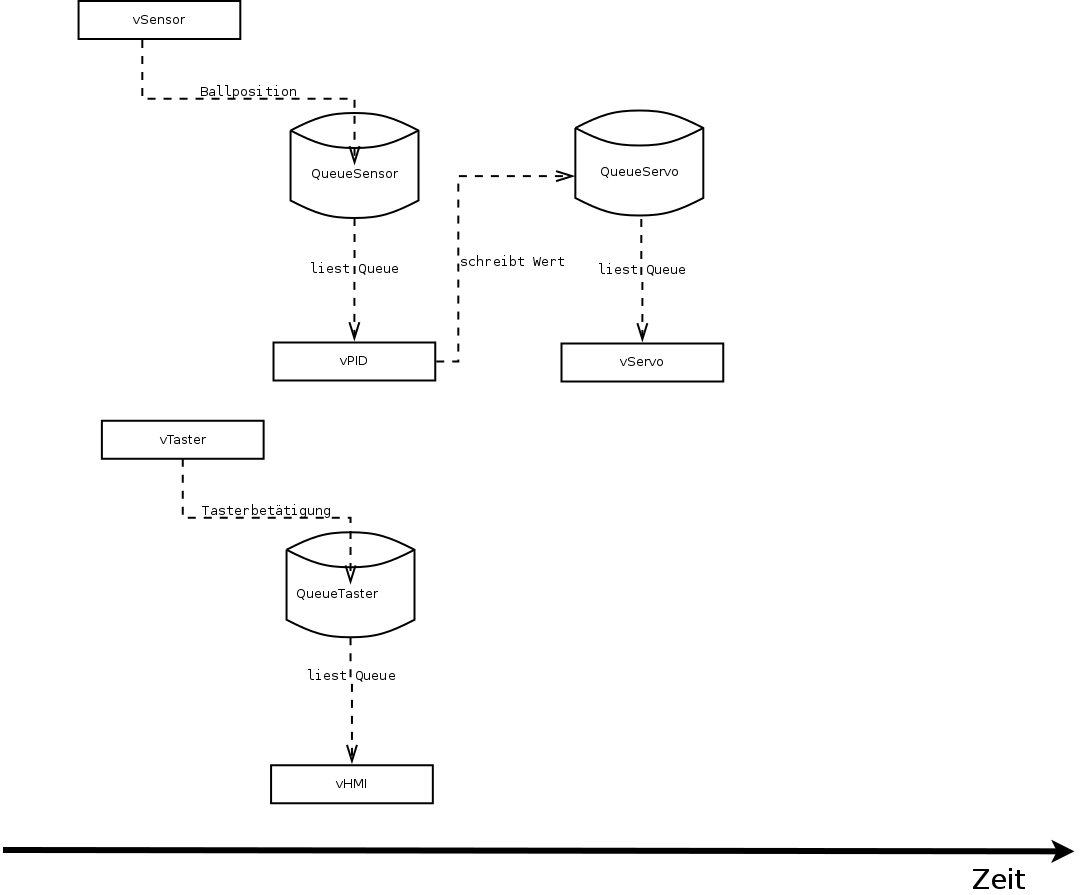
\includegraphics[scale=0.4]{UML.png}

\subsection{Ergebnis}
Mit unseren aktualisierten PID-Werten ist es uns gelungen den Ball in weniger als zehn Sekunden an der gewünschten Stelle stehen bleiben zu lassen.\\

\subsection{Fazit}
Der Unterschied von der Simulation aus $Versuch\ 2$ zum tatsächlichen Modell in $Versuch\ 3$ ist sehr enorm. Allerdings haben wir ein kontinuierliches System modelliert und ein diskretes System im Modell vorgefunden. Alleine dieser Unterschied führt schon zu sehr unterschiedlichen Parametern des PID-Reglers. In der Simulation hätten wir dieses Problem erkennen und modellieren können. \\
Die äußeren Einflüsse auf das Modell sind allerdings nur sehr schwer zu modellieren. Man sollte sich immer bewusst sein, dass eine Simulation nicht zu 100 Prozent dem Modell entspricht und es vermutlich immer Abweichungen geben wird. \\
Nichtsdestotrotz hat uns die Versuchsreihe sehr viel Spass gemacht und es ist ein gutes Gefühl, wenn der Ball am Ende auf der gewünschten Position liegen bleibt.